% Begin ims-style.tex ----------------------------------------------------------

% Output formats ---------------------------------------------------------------

% PDF

%\usepackage[bookmarksnumbered, pdfborder = {0 0 0}, urlcolor = oiGB, colorlinks = true, linkcolor = oiGB, citecolor = oiGB, backref = true]{hyperref}
% Including this gives error: Option clash for package hyperref

% Packages ---------------------------------------------------------------------

\usepackage[framemethod=tikz]{mdframed} 
\usepackage[normalem]{ulem}
\usepackage{subfigure}
\usepackage[explicit]{titlesec}
\usepackage{
  amsmath, calc,
  footnote, fancyhdr,
  geometry, graphicx,
  makeidx,
  booktabs,
  longtable,
  array,
  multirow,
  wrapfig,
  float,
  colortbl,
  pdflscape,
  tabu,
  threeparttable,
  threeparttablex,
  makecell,
  xcolor
}
%\newcommand{\UnderscoreCommands}{%
%  \do\citep \do\citeP
%}
\usepackage[strings]{underscore} % must be last

% Colors -----------------------------------------------------------------------

\definecolor{oiB}{HTML}{569BBD}            % COL["blue","full"]
\definecolor{oiLB}{HTML}{d5e6ef}           % lighter version of oiB

\definecolor{oiY}{HTML}{f4dc00}            % COL["yellow","full"]
\definecolor{oiLY}{HTML}{fffacd}           % lighter version of oiY

\definecolor{oiR}{HTML}{E97583}            % COL["red","full"]
\definecolor{oiLR}{HTML}{F3CED4}           % lighter version of oiR

\definecolor{oiGray}{HTML}{808080}         % COL["gray","full"]
\definecolor{oiLGray}{HTML}{f8f8f8}        % lighter version of oiR

\definecolor{oiGB}{rgb}{0.5,0.5,.5}        % from OS4 - for footnotes

% Headers 

\fancypagestyle{plain}{%
\fancyhf{} % clear all header and footer fields
\fancyhead[RO,RE]{\thepage} %RO=right odd, RE=right even
\renewcommand{\headrulewidth}{0pt}
\renewcommand{\footrulewidth}{0pt}
\renewcommand{\footruleskip}{5pt}}
\raggedbottom

% Make index

\makeindex

% add space between table rows 

\setlength{\defaultaddspace}{10pt}

% footnotes - try to stop them from running accross two pages

\interfootnotelinepenalty=10000

%-------------------------------------------------------------------------------
% From OS4 style.tex
%
% 1 Page Parameters
% 1.1
\setlength\paperheight{11in}
\setlength\paperwidth{8.5in}
\newcommand{\officialtextheight}{9.7in}
\newcommand{\officialtextwidth}{6in}
%\setlength\paperheight{10in}
%\setlength\paperwidth{8in}
%\newcommand{\officialtextheight}{8.7in}
%\newcommand{\officialtextwidth}{6in}
\newcommand{\officialvoffset}{-0.6in}
\setlength\textheight{\officialtextheight}
\setlength\textwidth{\officialtextwidth}
\setlength\voffset{\officialvoffset}
\renewcommand{\baselinestretch}{1.0}

% 1.2 Margin Size
\setlength\hoffset{0.25in}
% 1.2.1 Even
\setlength\oddsidemargin{0in}
\setlength\evensidemargin{0in}
% 1.2.2 Slightly offset
%\setlength\oddsidemargin{0.08in}
%\setlength\evensidemargin{-0.08in}
% 1.2.3 Significant offset
% WARNING: The chapter pages will show partially hidden page numbers.
%\setlength\oddsidemargin{0.2in}
%\setlength\evensidemargin{-0.2in}
% 1.3 PDF Parameters
%\setlength\paperheight{11in}
%\setlength\textheight{8.25in}
%\setlength\paperwidth{8.5in}
%\setlength\textwidth{5.45in}
%\setlength\voffset{-10mm}
%\setlength\oddsidemargin{0.75in}
%\setlength\evensidemargin{0.75in}
% 1.4 Margin Spacing
\setlength{\marginparsep}{5mm}
\setlength{\marginparwidth}{20mm}

% 1.5 Page Header

\renewcommand{\headrulewidth}{0pt}
\fancyhead[RO,LE]{\thepage}
\fancyhead[RE]{\leftmark}
\fancyhead[LO]{\rightmark}
\fancyfoot[c]{}
\fancyheadoffset[RO,LE]{0.9in}

% 6.6 Hyperreferences
\newcommand{\oiRedirect}[2]{\href{http://www.openintro.org/redirect.php?go=#1&referrer=\referrer}{#2}}

% Chapter and section titles

\titleformat{\chapter}[display]
{\color{oiB}\normalfont\Huge\bfseries\fontfamily{phv}\selectfont}
{\color{oiB}Chapter \thechapter}{1em}{#1}

\titleformat{\section}
{\color{oiB}\normalfont\Large\bfseries\fontfamily{phv}\selectfont}
{\color{oiB}\thesection}{1em}{#1}

\titleformat{\subsection}
{\color{oiB}\normalfont\large\bfseries\fontfamily{phv}\selectfont}
{\color{oiB}\thesubsection}{1em}{#1}

\titleformat{\subsubsection}
{\color{oiB}\normalfont\normalsize\bfseries\fontfamily{phv}\selectfont}
{\color{oiB}\thesubsubsection}{1em}{#1}

% IMS specific style -----------------------------------------------------------

% Helper environments

% mdframedwithfootChapterintro: for chapterintro box
% currently none of them increment footnote counter,
% this seems to be the right approach?

\newenvironment{mdframedwithfootChapterintro}
{   
    \savenotes
    \begin{mdframed}[%
    topline=true, bottomline=true, linecolor=oiB, linewidth=1.4pt,
    rightline=false, leftline=false,
    backgroundcolor=oiLB]
    %\stepcounter{footnote} % don't increment footnote counter
    \renewcommand{\thempfootnote}{\arabic{footnote}}
    }
{
    \end{mdframed}
    \spewnotes
}

% mdframedwithfootGPWE: for guidedpractice and workedexample

\newenvironment{mdframedwithfootGPWE}
{   
    \savenotes
    \begin{mdframed}[%
    topline=true, bottomline=true, linecolor=oiB, linewidth=0.5pt,
    rightline=false, leftline=false,
    backgroundcolor=oiLGray]
    %\stepcounter{footnote}
    \renewcommand{\thempfootnote}{\arabic{footnote}}
    }
{
    \end{mdframed}
    \spewnotes
}

% mdframedwithfootImportant: for important

\newenvironment{mdframedwithfootImportant}
{   
    \savenotes
    \begin{mdframed}[%
    topline=true, bottomline=true, linecolor=oiR, linewidth=0.5pt,
    rightline=false, leftline=false,
    backgroundcolor=oiLGray]
    %\stepcounter{footnote}
    \renewcommand{\thempfootnote}{\arabic{footnote}}
    }
{
    \end{mdframed}
    \spewnotes
}

% mdframedwithfootTip: for tip, data, and pronunciation

\newenvironment{mdframedwithfootTipDataPro}
{   
    \savenotes
    \begin{mdframed}[%
    topline=true, bottomline=true, linecolor=oiGray, linewidth=0.5pt,
    rightline=false, leftline=false,
    backgroundcolor=oiLGray]
    %\stepcounter{footnote}
    \renewcommand{\thempfootnote}{\arabic{footnote}}
    }
{
    \end{mdframed}
    \spewnotes
}

% mdframedwithfootTutLab: for tutorials and labs

\newenvironment{mdframedwithfootTutLab}
{   
    \savenotes
    \begin{mdframed}[%
    topline=false, bottomline=false,
    rightline=false, leftline=false]
    \stepcounter{footnote}
    \renewcommand{\thempfootnote}{\arabic{footnote}}
    }
{
    \end{mdframed}
    \spewnotes
}


% Custom environments/boxes -------------------------------------------------------
% based on imsstyle.css

% uses regular mdframedwithfoot variants, might have footnotes

% chapterintro

\newenvironment{chapterintro}{
\vspace{4mm}
\begin{mdframedwithfootChapterintro}
\begin{minipage}[t]{0.10\textwidth}
{$\:$ \\ \setkeys{Gin}{width=2.5em,keepaspectratio}
\includegraphics{images/_icons/chapterintro.png}}
\end{minipage}
\hfill
\begin{minipage}[t]{0.90\textwidth}
\setlength{\parskip}{1em}
\large
}{\end{minipage}
\end{mdframedwithfootChapterintro}
\vspace{4mm}
}

% guidedpractice

\newenvironment{guidedpractice}{
\vspace{4mm}
\begin{mdframedwithfootGPWE}
\begin{minipage}[t]{0.10\textwidth}
{$\:$ \\ \setkeys{Gin}{width=2.5em,keepaspectratio}
\includegraphics{images/_icons/guided-practice.png}}
\end{minipage}
\hfill
\begin{minipage}[t]{0.90\textwidth}
\vspace{-2mm}
\setlength{\parskip}{1em}
\noindent\textbf{\color{oiB}\small\fontfamily{phv}\selectfont{\MakeUppercase{Guided Practice}}} $\:$ \\ \\
}{\end{minipage}
\end{mdframedwithfootGPWE}
\vspace{4mm}
}

% workedexample

\newenvironment{workedexample}{
    \let\oldrule\rule
    \renewcommand{\rule}[2]{\vspace{-2mm}\oldrule{##1}{##2}\vspace{-2mm}}
\vspace{4mm}
\begin{mdframedwithfootGPWE}
\begin{minipage}[t]{0.10\textwidth}
{$\:$ \\ \setkeys{Gin}{width=2.5em,keepaspectratio}
\includegraphics{images/_icons/worked-example.png}}
\end{minipage}
\hfill
\begin{minipage}[t]{0.90\textwidth}
\vspace{-2mm}
\setlength{\parskip}{1em}
\noindent\textbf{\color{oiB}\small\fontfamily{phv}\selectfont{\MakeUppercase{Example}}} $\:$ \\ \\
}{\end{minipage}
\end{mdframedwithfootGPWE}
\vspace{4mm}
}

% important

\newenvironment{important}{
    \let\oldtextbf\textbf
    \renewcommand{\textbf}[1]{{\textcolor{oiR}{\oldtextbf{##1}}}}
\vspace{4mm}
\begin{mdframedwithfootImportant}
\begin{minipage}[t]{0.10\textwidth}
{$\:$ \\ \setkeys{Gin}{width=2.5em,keepaspectratio}
\includegraphics{images/_icons/important.png}}
\end{minipage}
\hfill
\begin{minipage}[t]{0.90\textwidth}
\vspace{-2mm}
\setlength{\parskip}{1em}
}{\end{minipage}
\end{mdframedwithfootImportant}
\vspace{4mm}
}

% tip

\newenvironment{tip}{
\vspace{4mm}
\begin{mdframedwithfootTipDataPro}
\begin{minipage}[t]{0.10\textwidth}
{$\:$ \\ \setkeys{Gin}{width=2em,keepaspectratio}
\includegraphics{images/_icons/tip.png}}
\end{minipage}
\hfill
\begin{minipage}[t]{0.90\textwidth}
\vspace{-2mm}
\setlength{\parskip}{1em}
}{\end{minipage}
\end{mdframedwithfootTipDataPro}
\vspace{4mm}
}

% data

\newenvironment{data}{
\vspace{4mm}
\begin{mdframedwithfootTipDataPro}
\begin{minipage}[t]{0.10\textwidth}
{$\:$ \\ \setkeys{Gin}{width=2em,keepaspectratio}
\includegraphics{images/_icons/data.png}}
\end{minipage}
\hfill
\begin{minipage}[t]{0.90\textwidth}
\vspace{-2mm}
\setlength{\parskip}{1em}
}{\end{minipage}
\end{mdframedwithfootTipDataPro}
\vspace{4mm}
}

% pronunciation

\newenvironment{pronunciation}{
\vspace{4mm}
\begin{mdframedwithfootTipDataPro}
\begin{minipage}[t]{0.10\textwidth}
{$\:$ \\ \setkeys{Gin}{width=2em,keepaspectratio}
\includegraphics{images/_icons/pronunciation.png}}
\end{minipage}
\hfill
\begin{minipage}[t]{0.90\textwidth}
\vspace{-2mm}
\setlength{\parskip}{1em}
}{\end{minipage}
\end{mdframedwithfootTipDataPro}
\vspace{4mm}
}


% uses regular mdframed, won't have footnotes

% singletutorial

\newenvironment{singletutorial}{
\vspace{4mm}
\begin{mdframed}[topline=false, bottomline=false, rightline=false, leftline=false]
\begin{minipage}[t]{0.10\textwidth}
{$\:$ \\ \setkeys{Gin}{width=2em,keepaspectratio}
\includegraphics{images/_icons/singletutorial.png}}
\end{minipage}
\hfill
\begin{minipage}[t]{0.90\textwidth}
\vspace{-2mm}
\setlength{\parskip}{1em}
}{\end{minipage}
\end{mdframed}
\vspace{4mm}
}

% alltutorials

\newenvironment{alltutorials}{
\vspace{4mm}
\begin{mdframed}[topline=false, bottomline=false, rightline=false, leftline=false]
\begin{minipage}[t]{0.10\textwidth}
{$\:$ \\ \setkeys{Gin}{width=2em,keepaspectratio}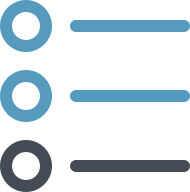
\includegraphics{images/_icons/alltutorials.png}}
\end{minipage}
\hfill
\begin{minipage}[t]{0.90\textwidth}
\vspace{-2mm}
\setlength{\parskip}{1em}
}{\end{minipage}
\end{mdframed}
\vspace{4mm}
}

% singlelab

\newenvironment{singlelab}{
\vspace{4mm}
\begin{mdframed}[topline=false, bottomline=false, rightline=false, leftline=false]
\begin{minipage}[t]{0.10\textwidth}
{$\:$ \\ \setkeys{Gin}{width=2em,keepaspectratio}
\includegraphics{images/_icons/singlelab.png}}
\end{minipage}
\hfill
\begin{minipage}[t]{0.90\textwidth}
\vspace{-2mm}
\setlength{\parskip}{1em}
}{\end{minipage}
\end{mdframed}
\vspace{4mm}
}

% alllabs

\newenvironment{alllabs}{
\vspace{4mm}
\begin{mdframed}[topline=false, bottomline=false, rightline=false, leftline=false]
\begin{minipage}[t]{0.10\textwidth}
{$\:$ \\ \setkeys{Gin}{width=2em,keepaspectratio}
\includegraphics{images/_icons/alllabs.png}}
\end{minipage}
\hfill
\begin{minipage}[t]{0.90\textwidth}
\vspace{-2mm}
\setlength{\parskip}{1em}
}{\end{minipage}
\end{mdframed}
\vspace{4mm}
}


% todo

\newenvironment{todo}{
\vspace{4mm}
\begin{mdframed}[%
    topline=true, bottomline=true, linecolor=oiY, linewidth=0.5pt,
    rightline=false, leftline=false,
    backgroundcolor=oiLY]
\begin{minipage}[t]{0.10\textwidth}
{$\:$ \\ \setkeys{Gin}{width=2em,keepaspectratio}
\includegraphics{images/_icons/to-do.png}}
\end{minipage}
\hfill
\begin{minipage}[t]{0.90\textwidth}
\vspace{-2mm}
\setlength{\parskip}{1em}
\noindent\textbf{\color{oiGray}\small\fontfamily{phv}\selectfont{\MakeUppercase{TO DO}}} $\:$ \\ \\
}{\end{minipage}
\end{mdframed}
\vspace{4mm}
}

% underconstruction

\newenvironment{underconstruction}{
\vspace{4mm}
\begin{mdframed}[%
    topline=true, bottomline=true, linecolor=oiR, linewidth=0.5pt,
    rightline=false, leftline=false,
    backgroundcolor=oiLR]
\begin{minipage}[t]{0.10\textwidth}
{$\:$ \\ \setkeys{Gin}{width=2em,keepaspectratio}
\includegraphics{images/_icons/under-construction.png}}
\end{minipage}
\hfill
\begin{minipage}[t]{0.90\textwidth}
\vspace{-2mm}
\setlength{\parskip}{1em}
\noindent\textbf{\color{oiR}\small\fontfamily{phv}\selectfont{\MakeUppercase{Under construction}}} $\:$ \\ \\
}{\end{minipage}
\end{mdframed}
\vspace{4mm}
}

% Cover image ------------------------------------------------------------------

\newenvironment{authorinfo}[1]
  {
  \begin{minipage}[c]{0.30\textwidth}
  {\setkeys{Gin}{width=12em,keepaspectratio}\includegraphics{#1}}
  \end{minipage} 
  \hfill
  \begin{minipage}[c]{0.60\textwidth}
  }
  {
  \end{minipage}
  }

% Part formatting --------------------------------------------------------------

\titleformat{\part}[display]
{\color{oiR}\titlerule[5pt]\vspace{3pt}\color{oiLR}\titlerule[2pt]\vspace{3pt}\color{oiB}\normalfont\Huge\bfseries\scshape\fontfamily{phv}\selectfont}
{\color{oiB}PART \thepart}{2em}{#1 \\ \noindent \vspace{3pt}\color{oiR}\titlerule[5pt]}

% https://tex.stackexchange.com/questions/506428/background-color-for-section-title
%\titleformat{\part}{\LARGE}{\rlap{\color{oiLB}\rule[-0.4cm]{\linewidth}{5cm}}\color{oiB}\normalfont\Huge\bfseries\scshape\fontfamily{phv}\selectfont PART \thepart}{1em}{\color{oiB}\normalfont\Huge\bfseries\scshape\fontfamily{phv}\selectfont #1}


% Bibliography: Chapter should be called References ----------------------------

% need to add this

% End ims-style.tex ------------------------------------------------------------